\documentclass[Report.tex]{subfiles}
\externaldocument[I-]{chapter_1_introduction}
\externaldocument[D-]{chapter_3_discardMethod}
\externaldocument[R-]{chapter_4_result}
\externaldocument[C-]{chapter_5_conclusion}
\externaldocument[RE-]{chapter_6_recognition}


\begin{document}
\chapter{Method}
\label{sec:Method}
\section{Description}
%The following section as described in Section~\ref{I-subsec:Report Layout} will
present our methods. Bellow we present each component individually and the
corresponding methods for them. A short description on what challenges have to
be solved for each component will be addressed first. \\ \\


\section{Component: Text segmentation}
\label{Method:Text_segmentation}

\subsection{Description}
In this part of the program, we want to be able segment out parts of text in the image. We want to then later segment out lines and letter for further classification. In this part wee assume that the image will mainly black text on white paper.

\subsection{Tried}
We where uncertain on how to do this part when we initial started the project. We ended up looking for a lot of different ways to do this part. We ended up trying 3 different approaches with mix result.
\begin{enumerate}
  \item Simple image analysis technics, using Otsu thresholding and Morphology.(Used)
  \item Stroke Width Transform(SWT) to detect text in natural images.(Discarded)
  \item OpenCv implementation of Scene Text Detection.(Discarded)
\end{enumerate}

\begin{flushleft}
  \subsubsection{Approach 1: Simple Image Analysis Technics}
  We was inspired by the this online blog \href{https://www.danvk.org/2015/01/07/finding-blocks-of-text-in-an-image-using-python-opencv-and-numpy.html}{Source}\cite{_finding_????}. We simplified the original approach to the following steps:
  \begin{enumerate}
    \item \textbf{Find Edges/Outliners of the image.}
    Initial idea is to use Canny, but we found Morphological Gradient to perform better. It indicates the contrast of the edges, so we can get better differences in some natural images.(so long the text and background is close to black and white)
    \item \textbf{Otsu Thresholding.}
    We need our image to be a binary image. We simply use OpenCV Otsu algorithm to achieve it.
    \item \textbf{Morphological Closing.}
    Since we want line segments we used Morphological Closing with large horizontal filter to merge as many horizontal letter together as possible.
    \item \textbf{Extract Regions}
    OpenCv FindContours was used to find the different text regions. We then exclude any regions that is smaller than a selected threshold. The different region are return as coordinate of the different rectangular boxes.
  \end{enumerate}
\end{flushleft}

\begin{flushleft}
  \subsubsection{Approach 2: Stroke Width Transform}
  The second approach we tried Stroke Width Transform to do Text Segmentation, it was original propose by Epstein et al 2010 \cite{epshtein_stroke_2010}. Since OpenCv do not have this implemented we tried to implement it ourself. Additional sources was used in our attempt to implement it\cite{werner_text_????, _c++_????, bunn_strokewidthtransform:_2018}. We was not able to finish this, but think we should mention it since we spend some time on it. The steps of Stroke Width Transform is as followed:
  \begin{enumerate}
    \item \textbf{Edge Detection and edge orientation(Done)}
    We need to have Edge image and orientation of the gradient image.
    Canny and Sobel was used in the original paper and other sources. This is simple since OpenCv have both Canny and Sobel implemented.
    \item \textbf{Stroke Width Transform(Done)}
    Here we had to do more. We have to find a line from a starting point and the angle. We was able to implement this part, but was some uncertainties. It only work on black text with white background. That is because the orientation(Sobel filtering) are dependent on it. The paper talk about doing a second pass with inverse image, but we decided to ignore it, in order to come farther in the algorithm.
    \item \textbf{Find Connected Component(Done)}
    In this point we are to connect component with the same Stride length together. We used One component at a time algorithm to find all the different components. We was able to finish it.
    \item \textbf{Exclude noise and find letters(not Done)}
    Since Stroke Width Transform tend to make a lot of noise. The obvious one is making single lines. This part are suppose to exclude this noise and at the same time exclude anything that is not a letter.The theory is, since letter and text all usually have the same stroke width, we can use this information do estimate what is letter and what is not. We was not able to finish this part.
    \item \textbf{Find lines/words(not Done)}
    Was not able to get to this part, but ideal it will combine letters to a single line or words.
  \end{enumerate}
  In cases where the image have a lot of non text object, it will work fine with it. We ended up discarding this approach since it was to time consuming and decided on working on simple approach first.
\end{flushleft}

\begin{flushleft}
  \subsubsection{Approach 3: OpenCv Scene Text Detection}
  OpenCV have it own Text Scene Detection. The approach of this algorithm is to detect text in scene using Classifier and Components Tree, propose by Lukás Neumann \& Jiri Matas \cite{neumann_real-time_2012}. Since we already discarded Stroke Width Transform to focus on simple approach, we decided not use it. We had some problem to get propel result as well.
\end{flushleft}

\subsection{Used in end result}
Since we had problem on getting with both approach 2 and 3 we decided on approach 1. It gave us ideal result on most images, but have some problem in images with non text objects.

\todo{fill the figure with good examples}
\begin{figure}[h]
  \centering
  \begin{subfigure}[t]{4cm}
    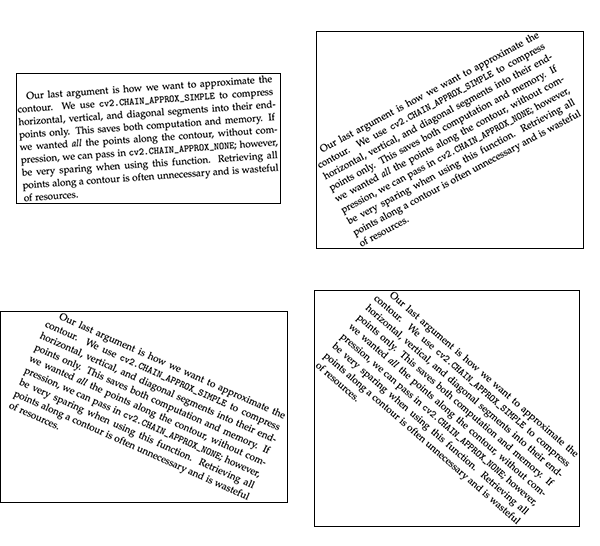
\includegraphics[width=3cm]{res/segment_text1.png}
    \caption{Example 1, Good result on just text}
  \end{subfigure}
  \hspace{5mm}%
  \begin{subfigure}[t]{4cm}
    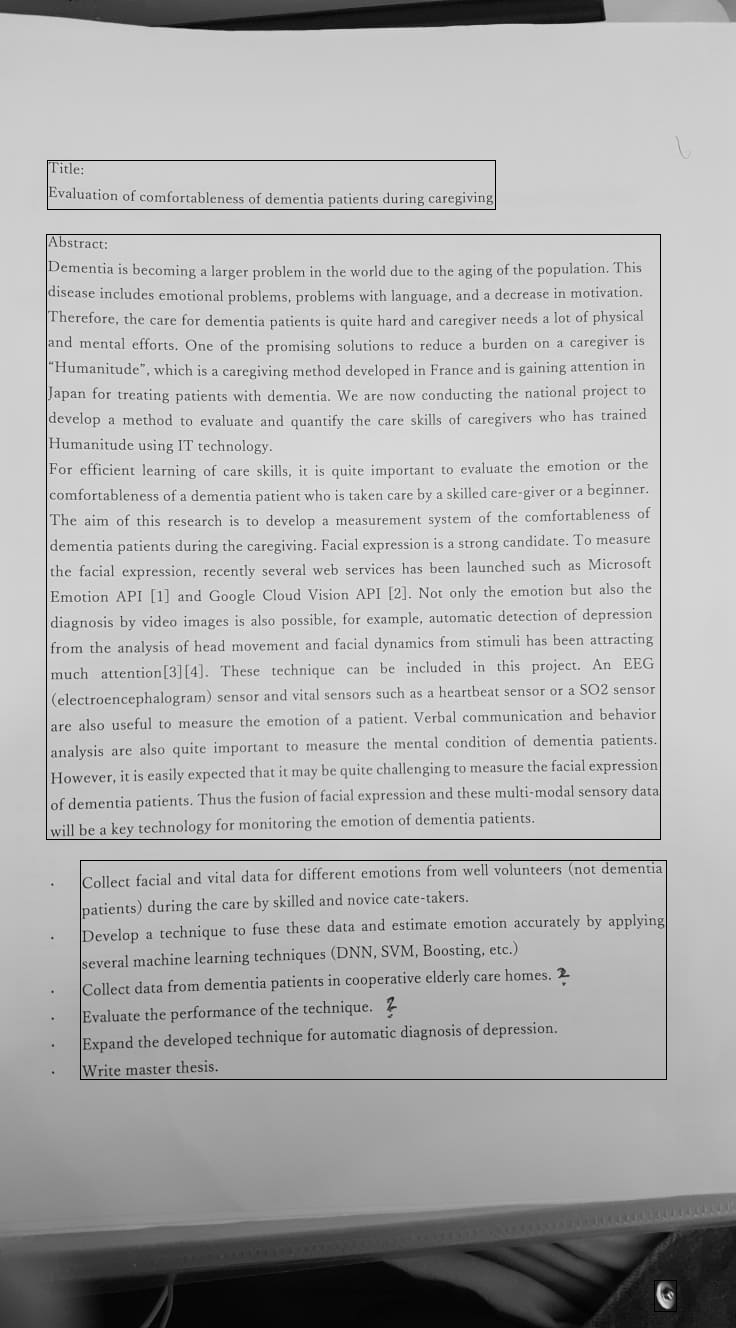
\includegraphics[width=3cm]{res/segment_text2.png}
    \caption{Example 2, Good result on paper}
  \end{subfigure}
  \hspace{5mm}%
  \begin{subfigure}[t]{4cm}
    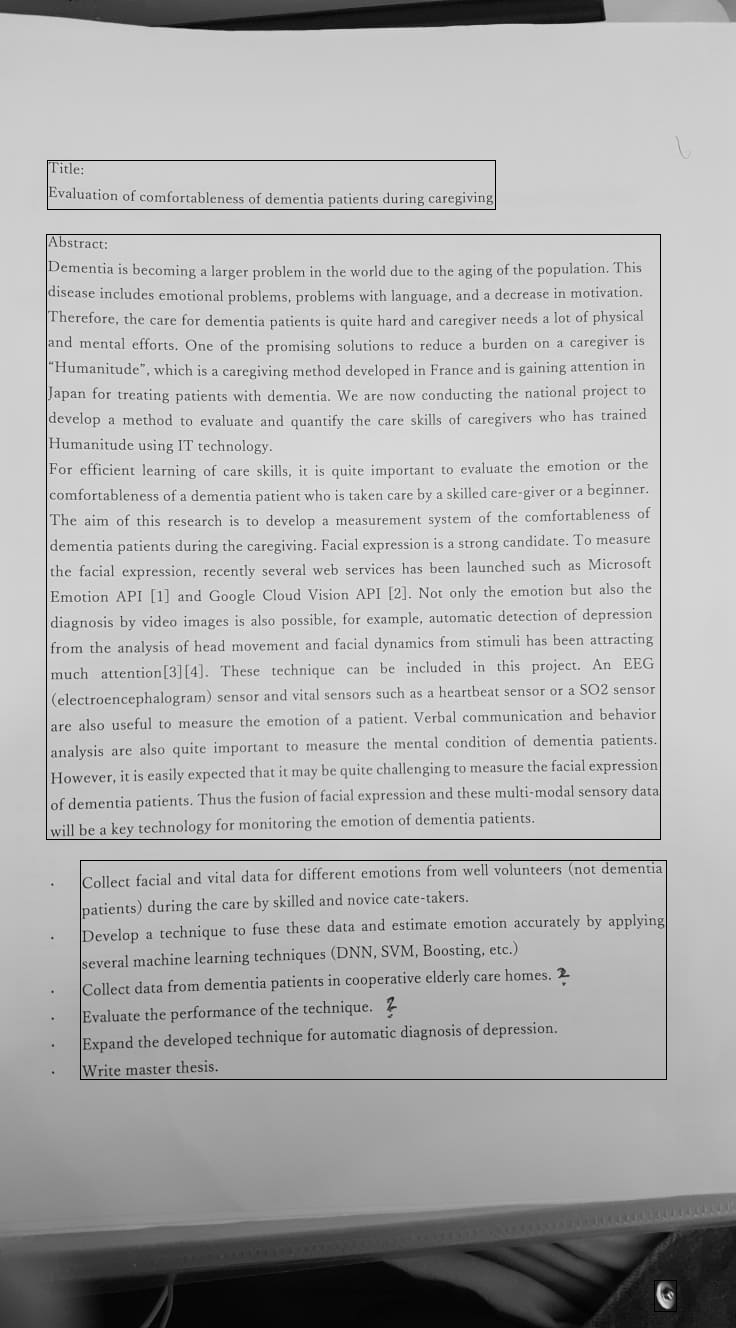
\includegraphics[width=3cm]{res/segment_text3.png}
    \caption{text}
  \end{subfigure}
  \caption{Example 3, Part of the text was not included}
  \label{fig:Text_detection_approaches}
\end{figure}










\section{Component: Preprocessing}
\label{Method:Preprocessing}
\subsection{Description}
Definition of preprocessing; the act of preparing the data for further use,
in our case for classification. \par
After the text segmentation we assume we have an image consisting of only text
in black, and background in white. What remains for us to do is to segment out
each character and format it to the right datatype for the classifier. Hence
the challenges we will have to solve here are:


\begin{flushleft}
  \textbf{Challenges}
  \begin{itemize}
    \item{Data formating/casting}
    \begin{itemize}
      \item{The data we want to test a classifier on needs to match the data we trained our classifier with. Hence we need to format our data to the same format as the datasets. No need for a specific approach.}
    \end{itemize}
    \item{Rotated text}
    \begin{itemize}
      \item{Our approach for character segmentation needs text rotated horisontally.}
    \end{itemize}
      \item{Line segmentation}
    \begin{itemize}
      \item{Our approach for character segmentation needs lines as input, as a sequence of lines on top of eachother breaks the algorithm.}
    \end{itemize}
      \item{Character segmentation}
    \begin{itemize}
      \item{We need to segment each character because the classifier cannot distingush several characters from one image.}
    \end{itemize}
  \end{itemize}
\end{flushleft}


\subsection{Find rotation}
\begin{flushleft}
  \textbf{Approach: OpenCV minAreaRect() + CNN solution} \\
  This approach uses \href{https://en.wikipedia.org/wiki/Convex_hull}{convex hull}
  to find the convex hull of the text segments, and then
  \href{https://en.wikipedia.org/wiki/Rotating_calipers}{rotating calipers} to
  find the minimum Area rectangle. \par
  One important note here is that this method only works if the images sent as
  input is binary. Because we want the convex hull algorithm to find the convex
  hull of the text segment. \par
  This method is really good at finding the angles, however it does not solve the
  problem of rotating the text correctly, Figure~\ref{fig:4angle_rot} illustrates
  this problem. It will only allow us to rotate it along one of the text
  segments edges. To rotate the text correctly from the result of cv.minAreaRect
  we used an approach using Convolutional neural networks.

  \begin{enumerate}
    \item \textbf{Binary image}
    For the Convex hull algorithm to work, the text segment and the background
    needs to be distinguishable. Convert image to a binary image.
    \item \textbf{cv.minAreaRect()}
    Run the minAreaRect() method.
    \item \textbf{Custom CNN solution - find correct rotation}
    Now that we have one of [0\textdegree, 90\textdegree, 180\textdegree,
    270\textdegree], we run a character classification on a subset of the
    entire text. Next the classifier which returns an angle which has the
    highest probobility, we set as the true angle, we rotate the text
    accordingly.
  \end{enumerate}
\end{flushleft}


\subsection{Find line}


\subsection{Find Symbol/Letter Segmentation}
Letter segmentation was similar to Text Segmentation. we added a few steps and removed the morphology part. The additional step was to fill holes in the image, example like 8 and O can give multiple wrong contour. cv2.floodFill was used to solve this problem.
\begin{enumerate}
  \item Do threshold.
  \item Inverse the image since we work on black text on white background.
  \item Fill any holes, cv2.floodFills
  \item FindContours
\end{enumerate}
\subsection{Approach: find contour after Filled holes}
test text alksjdfh alsjkdbfkas


\section{Component: Classification}
\label{Method:Classification}
\begin{flushleft}
  \textbf{Description} \\
  For the classification component there where only 2 approaches we considered,
  Convolutional Neural Network (CNN), the architecture is illustration in
  Figure~\ref{fig:CNN_architecture}, and a Multilayer Perceptron (MLP or Deep
  neural network (DNN)), Figure~\ref{fig:neural_net2}. However the method we
  ended up choosing for the final result is CNN. In
  Section~\ref{D-sec:Discarded Method:Classification} we explain why we discarded
  the MLP approach. \par
\end{flushleft}

\begin{flushleft}
  \textbf{Convolutional Neural Network} \\
  Convolutional neural networks are especially good for image
  classification, because they take local spatial connections into account when
  they classify. This way it doesn't matter where in the image our
  object/character is it will be able to recognize it, same yields for rotation,
  as the CNN classifies based on local spatial connections it doesn't matter if
  the object is rotated. Hence the classification would be even more robust
  compared to the MLP. \par
  The basic idea of a CNN is somewhat understood, but the algorithms and how to
  implement it is still not 100\% grasped. Hence because of lack of knowledge,
  trying to solve the classification problem with a CNN will mostly be done
  by researching and trying to solve it as it unfolds.
\end{flushleft}

\begin{figure}[H]
  \centering
  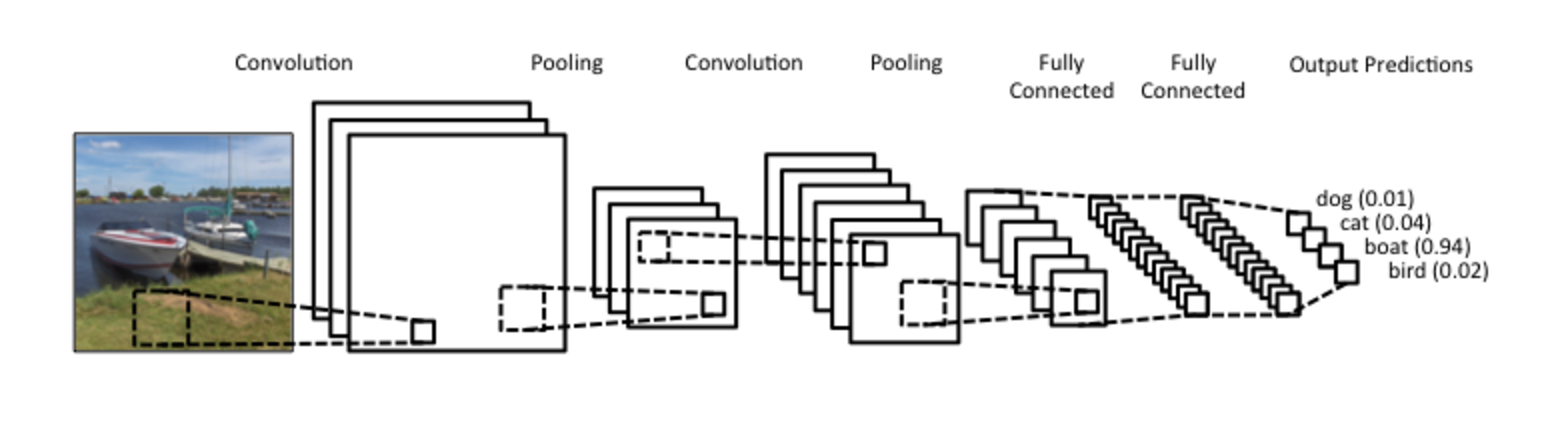
\includegraphics[height=4cm]{res/CNN_architecture.png}
  \caption{Convolutional Neural network \href{ http://www.wildml.com/2015/11/understanding-convolutional-neural-networks-for-nlp/}{Source}}
  \label{fig:CNN_architecture}
\end{figure}

\begin{flushleft}
  \textbf{CNN - Basics} \\
  \begin{itemize}
   \item{Convolutional layer}
   \begin{itemize}
    \item{This layer consists of several filters/kernels that are convolved over
    the image and based on how many filters one uses, the same amount of feature
    images are made. The purpose of the filters are to grasp some spatial
    characteristics of the image, and make it available for further processing.
    The filters here correspond to the weights in the MLP, these are first
    initialized at random (or with a smart initialization method), then these
    will be updated as the network is trained. Some features that the filters
    might find could be; vertical or horizontal lines, they could also find more
    complex features like faces or animals at later layers. \par
    In a CNN we can have arbitrary many convolutional layer and arbitrary many
    filters at each layer. However just like a regular MLP, increasing the
    number of layers and or filters; can allow the network to fit the training
    data arbitrarily well, unfortunately at the cost of processing time.}
   \end{itemize}
   \item{Pooling}
   \begin{itemize}
    \item{The pooling layer allows us to downsize the data. This makes it
    possible to start with data which are relatively big, and as the data propagates
    through the network we downsize it. As for the convolution layer the pooling
    layer can be used arbitrarily many times in a network.}
   \end{itemize}
   \item{Fully connected layers (FC)}
   \begin{itemize}
    \item{This layer works basically the same way as the hidden layers in an MLP.
    The pixels of the image is sent as data for each node and they propagate
    through these layers (usually 2 layers of FC are used) just as they would in
    an MLP.}
   \end{itemize}
  \end{itemize}
\end{flushleft}


\section{Component: Datasets}
\label{Method:Datasets}
\subsection{Description}

\begin{flushleft}
  \textbf{Description} \\
  Labeled data is needed because our classifiers need to be trained to understand
  the difference between the characters. This is usually done by training a
  classifier with a set of training data, labels are needed in our case,
  since it is a supervised machine learning algorithm we want to use. As the
  training data is used to train the software, we will need data to test our
  software as well, hence the need for test data. The test data is used to get a
  measure of what the error rate of our software is, based on the results we
  can then tune the hyper-parameters to get a better/smaller error rate. Lastly
  we will need validation dataset. This is an independent dataset that the software
  is not familiar with. The accuracy of the software on the validation set will
  then be a measure of how good the software can classify the characters.
\end{flushleft}

\begin{flushleft}
  \textbf{Limitation - proof-of-concept} \\
  As we have limited us to the English alphabet and numbers ranging from [0-9],
  we will need labeled data for each of these 36 characters; training, test and
  validation sets. As the concept of classifying only numbers vs all 36
  characters does not differ that much, we will first see if we can solve the OCR
  problem with just numbers. Therefore we only need a dataset containing numbers
  at first. Thereafter we will search for a dataset containing all the characters
  we need.
\end{flushleft}

\begin{flushleft}
  \textbf{Dataset} \\
  \textbf{MNIST} \\
  This is a dataset containing handwritten numbers [0-9].
  It has a training set of 60.000 examples and a test set of 10.000 examples.
  (ref. reader to http://yann.lecun.com/exdb/mnist/).
\end{flushleft}





\newpage

\section{Classification}
\label{sec:Discarded Method:Classification}

\begin{flushleft}
  \textbf{Deep Neural Network} \\
  Multilayer perceptron neural networks are relatively straight
  forward to code, however the challenging part is to decide on good
  hyper-parameters and to not overfit our network. \par
  Research has shown that the choices of parameters can have huge effects on
  the error rate through empirical testing. As empirical testing has shown that
  some combinations of parameters are better than others, we will also use the
  same method to find decent values on several of the hyper-parameters. More on
  this bellow, where a short description of the hyper-parameters follow. \par
  One obvious disadvantage we might face by using MLP is that slight spatial
  change on where in the image the characters are located, might lead to
  characters classified differently. This is because there is no spatial
  connections on a MLP.
\end{flushleft}

\begin{figure}[H]
  \centering
  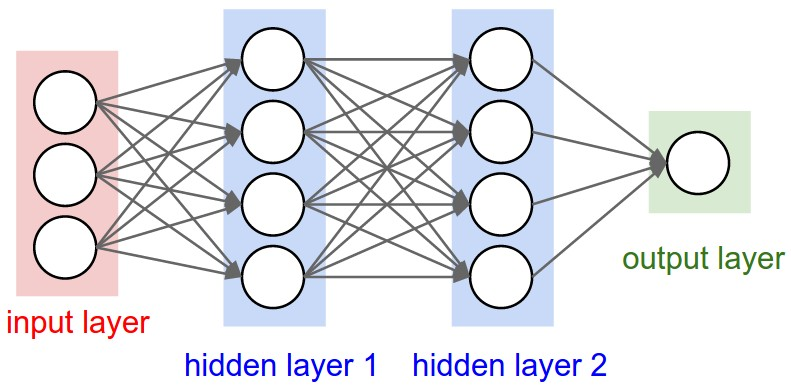
\includegraphics[height=4cm]{res/neural_net2.jpeg}
  \caption{MLP Neural network \href{http://cs231n.github.io/neural-networks-1/}{Source}}
  \label{fig:neural_net2}
\end{figure}


\begin{flushleft}
  \textbf{Hyper-parameters}
  \begin{itemize}
   \item{Number of hidden layers}
   \begin{itemize}
    \item{Layers decide how well the software can define the decision borders.
    Hence increase in layers can have a positive effect, there are also cons with
    the amount of layers. The more layers, the greater the computational power
    needed to train the system. We will be using the empirical method to decide
    how many layers we need}
   \end{itemize}
   \item{Number of nodes in each hidden layer}
   \begin{itemize}
    \item{Nodes in each hidden layer has the same effect as the number of hidden
    layers, hence the same applies for this hyper-parameter. }
   \end{itemize}
   \item{Activation functions}
   \begin{itemize}
    \item{The activation function decides which combination of nodes, with their
    signals, are allowed to propagate through the network. Here we will be using
    the \textit{rectified linear unit} (RELU) activation function. This is an
    activation function that allows propagation if the signal is positive,
    otherwise it will forward a zero. The reason for choosing this activation
    function is because this function handles the \textit{vanishing gradient
    problem} better than sigmoid and a tanh activation functions. More on
    vanishing gradient problem under ``optimization function''.}
   \end{itemize}
   \item{Loss function}
   \begin{itemize}
    \item{The loss function describes how far off the predicted class of the
    character is from the real class. In our case since we have multiple
    classes and we are going to use \textit{softmax regression} as the output
    layer, we also will be using the \textit{cross-entropy loss function}.}
   \end{itemize}
   \item{Optimization function}
   \begin{itemize}
    \item{The backpropogation will train the weights by Gradient Decent
    Optimization. However as training with several thousand examples, and then
    optimizing the weights and run the training process, is too costly resource
    wise, we will have to implement the \textit{mini-batch gradient decent
    optimizations}. Same principle as gradient decent optimization, but this way
    we will find the gradient decent for each batch. As long as these batches are
    randomly chosen, and the sizes are large enough, (we will be using 100 as
    batch size), these will represent the entire dataset well enough.}
   \end{itemize}
   \item{Learning rate}
   \begin{itemize}
    \item{Learning rate is a scalar that decides how large the steps towards
    the gradient minimum will be, for the weights. Choosing too small of a
    learning-rate we might risk not reaching the bottom of the graph, we also
    might get stuck in a local minimum. Choosing too large of a learning rate
    we might risk never settle down on a minimum. \par
    For the learning rate we will be using the empirical method too.}
   \end{itemize}
   \item{Initialization of the weights and biases}
   \begin{itemize}
    \item{Initialization of the weights also seems to be of importance,
    researchers have found out. This is obvious, as for example setting all the
    weights to zero, would of course lead to a network with very few active
    nodes. \par
    We will be using the initialization of zeros for the biases, not any
    apparent reason. Based on our research, it seems people have gotten decent
    results when using this initialization. For the weights we will be using a
    gaussian distribution, mean=0, standard deviation=1. Again this is also
    something that we have read should be a good initialization for the weights,
    no other reason.}
   \end{itemize}
   \item{Number of epochs}
   \begin{itemize}
    \item{Number of epochs are only relevant when we have a small number of
    dataset. When we have a small dataset we might want to run the software on
    the same dataset several times. This might result in overfitting the software
    to the dataset, therefore it is really important to be careful of the number of
    epochs, in cases with small datasets.}
   \end{itemize}
  \end{itemize}
\end{flushleft}


\section{Datasets}

\end{document}
